\documentclass[]{article}
\usepackage[top=1.3in,bottom=1.3in,left=1in,right=1in]{geometry}
\usepackage{tikz}
\usetikzlibrary{shapes.geometric,arrows.meta}
\usepackage[size=small]{caption}
\usepackage{xcolor}
\usepackage[colorlinks,allcolors=blue]{hyperref}
\usepackage[noabbrev]{cleveref}
\usepackage{multicol}
\usepackage{float}

\title{
    {\LARGE Project Part B}
    \\[1ex]
    {\Huge\bf Playing the Game}
}
\author{
    COMP30024 Artificial Intelligence
}
\date{2021}


% Custom TikZ commands
\newcommand{\hex}[4] {
    \node[hex,fill={#3}] at ({#1}, {#2}) {};
    \node[hex,thick,draw={#3},fill={#3!10}] at ({#1}, {#2}) {};
    \node at ({#1}, {#2}) {{#4}};
}
\newcommand{\uptoken}[3] {
    \node[draw,circle,minimum size=5.3mm,fill=white] at (#1, #2) {};
    \node[draw,circle,minimum size=4.2mm,very thick,black]  at (#1, #2) {};
    \node[] at (#1, #2) {#3};
}
\newcommand{\lotoken}[3] {
    \node[draw,circle,minimum size=5.3mm,fill=white] at (#1, #2) {};
    \node[draw,circle,minimum size=4.2mm,very thick,purple] at (#1, #2) {};
    \node[] at (#1, #2) {#3};
}
\newcommand{\board} {
    \tikzset{
        hex/.style={
            regular polygon,
            regular polygon sides=6,
            minimum size=7mm,
            inner sep=0mm,
            outer sep=0mm,
            rotate=30,
            draw
        },
        x={(3.031mm,5.25mm)},
        y={(6.062mm,0mm)}
    }
    \foreach \r/\q in {
                    +4/-4,+4/-3,+4/-2,+4/-1,+4/+0,
                 +3/-4,+3/-3,+3/-2,+3/-1,+3/+0,+3/+1,
              +2/-4,+2/-3,+2/-2,+2/-1,+2/+0,+2/+1,+2/+2,
           +1/-4,+1/-3,+1/-2,+1/-1,+1/+0,+1/+1,+1/+2,+1/+3,
        +0/-4,+0/-3,+0/-2,+0/-1,+0/+0,+0/+1,+0/+2,+0/+3,+0/+4,
           -1/-3,-1/-2,-1/-1,-1/+0,-1/+1,-1/+2,-1/+3,-1/+4,
              -2/-2,-2/-1,-2/+0,-2/+1,-2/+2,-2/+3,-2/+4,
                 -3/-1,-3/+0,-3/+1,-3/+2,-3/+3,-3/+4,
                    -4/+0,-4/+1,-4/+2,-4/+3,-4/+4,
    }
        \node[hex,fill=black!5] at (\r, \q) {};
}



\begin{document}

\maketitle


\section{Overview}
\label{sec:overview}

In this second part of the project, we will play the full two-player
version of \emph{RoPaSci~360}.
Before you read this specification you may wish to re-read the
`Rules for the Game of \emph{RoPaSci~360}' document.

The aims for Project Part B are for you and your project partner to
(1)~practice applying the game-playing techniques discussed in
    lectures and tutorials,
(2)~develop your own strategies for playing \emph{RoPaSci~360}, and
(3)~conduct your own research into more advanced algorithmic game-playing
    techniques;
all for the purpose of creating the best \emph{RoPaSci~360}--playing
program the world has ever seen.

\begin{figure}[ht!]
    \centering
    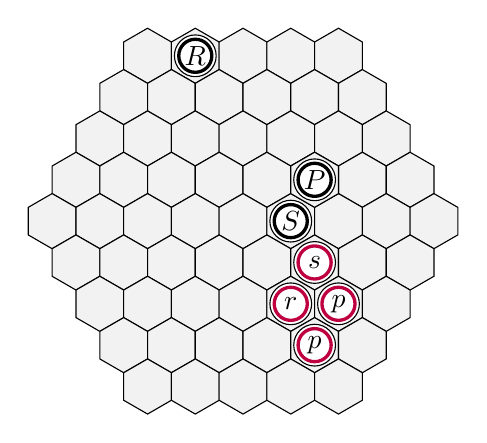
\begin{tikzpicture}
        \board
        \uptoken{+4}{-3}{$R$}
        \uptoken{+1}{+1}{$P$}
        \uptoken{+0}{+1}{$S$}
        \lotoken{-1}{+2}{$s$}
        \lotoken{-2}{+2}{$r$}
        \lotoken{-2}{+3}{$p$}
        \lotoken{-3}{+3}{$p$}
    \end{tikzpicture}
\end{figure}

\subsection{The task}

Your task is twofold.
%
Firstly, you will \textbf{design and implement a program} to play the
game of \emph{RoPaSci~360}.
That is, given information about the evolving state of the game, your
program will decide on an action to take on each of its turns
(we provide a driver program to coordinate a game of \emph{RoPaSci~360}
between two such programs so that you can focus on implementing the
game-playing strategy).
%
\Cref{sec:program} describes this programming task in detail, including
information about how our driver program will communicate with your
player program and how you can run the driver program.

Secondly, you will \textbf{write a report} discussing the strategies your
program uses to play the game, the algorithms you have implemented, and
other techniques you have used in your work, highlighting the most
impressive aspects.
%
\Cref{sec:report} describes the intended structure of this document.

The rest of this specification covers administrative information about
the project.
%
For assessment criteria, see \Cref{sec:assessment}.
%
For submission and deadline information see \Cref{sec:submission}.
%
Please seek our help if you have any questions about this project.



\newpage

\section{The program}
\label{sec:program}

You must create a program in the form of a Python 3.6 \textbf{module}
named with \textbf{your team name}.


\subsection{\texorpdfstring{The \texttt{Player} class}{The Player class}}

When imported, your module must define a class named \texttt{Player}
with at least the following three methods:

\begin{enumerate}
    \item
        \texttt{def\ \_\_init\_\_(self,\ player):}
        Called once at the beginning of a game to initialise your player.
        Use this opportunity to set up an internal representation of the
        game state.

        The parameter \texttt{player} will be
        the string \texttt{"upper"} (if your program will play as Upper),
        or the string \texttt{"lower"} (if your program will play as Lower).
    \item
        \texttt{def\ action(self):}
        Called at the beginning of each turn. 
        Based on the current state of the game, your program should select
        and return an action to play this turn.

        The action must be represented based on the instructions
        for representing actions in the next section.
    \item
        \texttt{def\ update(self,\ opponent\_action,\ player\_action):}
        Called at the end of each turn to inform your player of both
        players' chosen actions.
        Use this opportunity to update your internal representation of the
        game state.

        The parameter \texttt{opponent\_action} will be your opponent's
        chosen action, and \texttt{player\_action} will be the same action
        your player just returned through the
        \texttt{action} method.
        %
        Both actions will be represented following the instructions for
        representing actions in the next section. The actions will always
        be allowed for the player 
        (your method \emph{does not} need to validate the actions against
        the game rules).
\end{enumerate}


\subsection{Representing actions}

\begin{multicols}{2}
Our programs will need a consistent representation for actions. We will
represent all actions as \emph{three-tuples} containing first a string
\textbf{action type} and then two \textbf{action arguments}, indexing
hexes with the \emph{axial coordinate system} from Part A
(see \Cref{fig:coordinates}).

\begin{itemize}
    \item
        To represent a \textbf{throw action}, use a tuple:
        \begin{center}
            \texttt{("THROW", $s$, ($r$, $q$))}
        \end{center}
        where
            $s$ is a string (\texttt{"r"} for rock, \texttt{"p"} for paper,
            or \texttt{"s"} for scissors, always in lower case) representing
            the symbol of token to throw, and
            $(r, q)$ are the coordinates of the token.

    \item
        To represent a \textbf{slide action} or a \textbf{swing action},
        use a tuple:
        \begin{center}
            \texttt{($atype$, ($r_a$, $q_a$), ($r_b$, $q_b$))}
        \end{center}
        where
        $atype$ is the action type (\texttt{"SLIDE"} or \texttt{"SWING"}),
        $(r_a, q_a)$ are the coordinates of the moving token before the
        action, and $(r_b, q_b)$ are the new coordinates.
\end{itemize}

% For example, the tuple \texttt{("THROW",\ "r"\ (2,\ 3))} represents
% a throw action adding a rock token to the hex indexed $(2, 3)$.
% The tuple \texttt{("SLIDE",\ (0,\ 1),\ (-1,\ 1))} represents a slide
% action for a token occupying the hex $(0, 1)$ to the new hex $(-1, 1)$.

\begin{figure}[H]
    \centering
    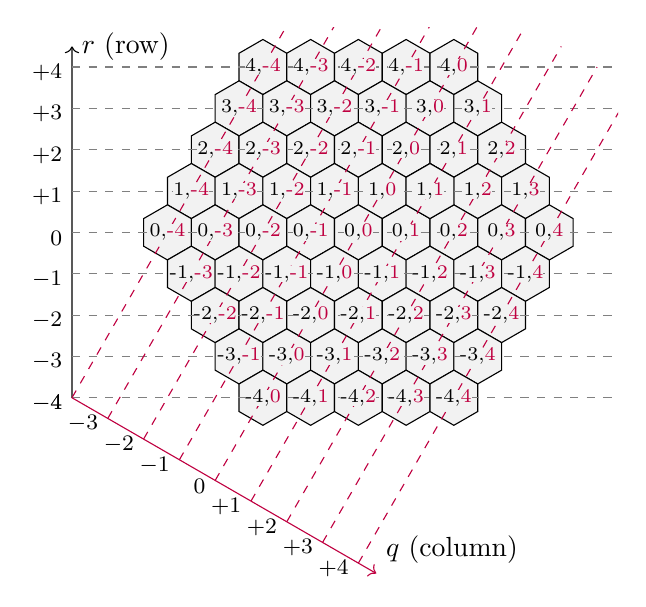
\begin{tikzpicture}
        \clip[] (-4.2, -4.4) rectangle (3.3, 2.6);
        \board
        % draw r axis
        \draw (-4, -4) edge[->] (4.5, -8.25);
        \node[right] at (4.5, -8.25)  {$r$ (row)};
        % draw q axis
        \draw (-4, -4) edge[->,purple] (-8.25, 4.5);
        \node[above right] at (-8.25, 4.5) {$q$ (column)};
        % draw dashed grid
        \foreach \i/\j in {0/-4,1/-3,2/-2,3/-1,4/0,5/+1,6/+2,7/+3,8/+4} {
            \node[left,yshift={-2pt}] at (\j, -4-0.5*\i) {\footnotesize $\j$};
            \draw (\j,-4-0.5*\i) edge[dashed,draw=gray] (\j,7.5-0.5*\i);
            \node[left,yshift={-2pt}] at (-4-0.5*\i, \j) {\footnotesize $\j$};
            \draw (-4-0.5*\i,\j) edge[dashed,draw=purple] (7.5-0.5*\i,\j);
        }
        % draw all points
        \foreach \r/\q in {4/-4,4/-3,4/-2,4/-1,4/0,3/-4,3/-3,3/-2,3/-1,3/0,
            3/1,2/-4,2/-3,2/-2,2/-1,2/0,2/1,2/2,1/-4,1/-3,1/-2,1/-1,1/0,1/1,
            1/2,1/3,0/-4,0/-3,0/-2,0/-1,0/0,0/1,0/2,0/3,0/4,-1/-3,-1/-2,
            -1/-1,-1/0,-1/1,-1/2,-1/3,-1/4,-2/-2,-2/-1,-2/0,-2/1,-2/2,-2/3,
            -2/4,-3/-1,-3/0,-3/1,-3/2,-3/3,-3/4,-4/0,-4/1,-4/2,-4/3,-4/4}
            \node[fill=black!5,inner sep=0pt] at (\r,\q)
                {\scriptsize \r,{\color{purple}\q}};
    \end{tikzpicture}
    \caption{
        \label{fig:coordinates}
        Each hex is addressed by a \textbf{row} ($r$) and \textbf{column}
        ($q$) pair, as shown.
        %
        For notes on a similar axial coordinate system, see
        \href
            {https://redblobgames.com/grids/hexagons}
            {\tt redblobgames.com/grids/hexagons/}
        (and \textbf{don't forget to acknowledge} any algorithms or
        code you use in your program).
    }
\end{figure}
\end{multicols}




\subsection{Running your program}

To play a game of \emph{RoPaSci~360} with your program, we provide a
driver program---a Python module called \texttt{referee}.
%
For your information, the referee program has the following essential
structure:
%
\begin{enumerate}
    \item
        Set up a \emph{RoPaSci~360} game.
        Initialise one \texttt{Player} class, as directed by the command
        line arguments, as each of Upper and Lower players
        (calling their \texttt{.\_\_init\_\_()} methods).
    \item
        Repeat the following until the game ends:
        \begin{enumerate}
            \item
                Ask each player for their next action
                (calling their \texttt{.action()} methods).
            \item
                Validate the actions and apply them to the game if they 
                are allowed
                (otherwise, end the game with an error message).
                Display the resulting game state to the user.
            \item
                Notify both players of the actions
                (calling their \texttt{.update()} methods).
        \end{enumerate}
    \item
        After detecting one of the ending conditions, display the
        final result of the game to the user.
\end{enumerate}

To play a game using \texttt{referee}, invoke it as follows.
%
The referee module (the directory \texttt{referee/}) and the modules with
your \texttt{Player} class(es) should be within your current directory:
%
\begin{quote}
    \texttt{python -m referee <upper module> <lower module>}
\end{quote}
%
where \texttt{python} is the name of a Python 3.6 interpreter\footnotemark
~and \texttt{<upper module>} and \texttt{<lower module>}
are the names of modules containing the classes \texttt{Player} to be used
for Upper and Lower, respectively.
% 
The referee offers many additional options.
% including for
% inserting a delay between turns (to make games easier to watch);
% controlling output verbosity; creating an action log; enforcing time
% constraints and (on linux) space constraints; configuring output style;
% and using other player classes (not named \texttt{Player}) from a module
% (useful for testing your main player against other player classes).
To read about them, run `\texttt{python~-m~referee~--help}'.

\footnotetext{
    \label{fn:dimefox}
    Note that Python 3.6 is not available on \texttt{dimefox} by default.
    However, it can be used after running the command
    `\texttt{enable-python3}' (once per login).
}

\subsection{Program constraints}

The following \textbf{resource limits} will be strictly enforced on
your program during testing.
%
This is to prevent your programs from gaining an unfair advantage
just by using more memory and/or computation time.
% 
These limits apply to each player for an entire game.
In particular, they \emph{do not} apply to each turn separately.
%
For help measuring or limiting your program's resource usage, see the
referee's additional options (\texttt{--help}).
%
\begin{itemize}
\item
  A maximum computation time limit of \textbf{60 seconds per player, per
  game}.
\item
  A maximum memory usage of \textbf{100MB per player, per game} (not
  including imported libraries).
\end{itemize}
%
You must not attempt to circumvent these constraints.
%
For example, do not use multiple threads or attempt to communicate
with other programs or the internet to access additional resources.

\subsection{Allowed libraries}

Your program should use \textbf{only standard Python libraries}, plus the
optional third-party libraries \textbf{NumPy and SciPy} (these are the
only libraries installed on dimefox).
With acknowledgement, you may also include code from the AIMA textbook's
Python library, where it is compatible with Python 3.6 and the above
limited dependencies.
%
Beyond these, \textbf{your program should not require any other libraries
in order to play a game}.

However, to develop your program, you may use \emph{any tools}, including
tools using other programming languages.
%
This is all allowed \emph{as long as your \texttt{Player} class does not
require these tools to be available when it plays a game}
(because they are not available on \texttt{dimefox}).

For example, let's say you want to use machine learning techniques to
improve your program.
%
You could use third-party Python libraries
such as scikit-learn/TensorFlow/PyTorch
to build and train a model.
%
You could then export the learned parameters of your model.
%
Finally, you would have to (re)implement the prediction component of the model
yourself, using only Python/NumPy/SciPy.
%
Note that this final step is typically simpler than implementing the
training algorithm, but may still be a significant task.



\section{The report}
\label{sec:report}

Finally, you must discuss the strategic and algorithmic aspects of your
game-playing program and the techniques you have applied in a separate
file called \texttt{report.pdf}.

This report is your opportunity to highlight your application of
techniques discussed in class and beyond, and to demonstrate the most
impressive aspects of your project work.

\subsection{Report structure}

You may choose any high-level structure of your report.
%
Aim to present your work in a logical way, using sections with clear
titles separating different topics of discussion.

Here are some suggestions for topics you might like to include in your
report.
%
Note: Not all of these topics or questions will be applicable to your
project, depending on your approach. That's completely normal. You should
focus on the topics which make sense for you and your work.
Also, if you have other topics to discuss beyond those listed here,
feel free to include them.
%
\begin{itemize}
    \item
        \textbf{Describe your approach:}
        %
        How does your game-playing program select actions throughout the
        game?

        Example questions:
        %
        What search algorithm have you chosen, and why?
        %
        Have you made any modifications to an existing algorithm?
        %
        How have you handled the simultaneous-play nature of this game?
        %
        What are the features of your evaluation function, and
        what are their strategic motivations?
        %
        If you have applied machine learning, how does this fit into
        your overall approach? What learning methodology have you followed,
        and why?
    \item
        \textbf{Performance evaluation:}
        %
        How effective is your game-playing program?

        Example questions:
        %
        How have you judged your program's performance? Have you compared
        multiple programs based on different approaches, and, if so, how
        have you selected which is the most effective?
    \item
        \textbf{Other aspects:}
        %
        Are there any other important creative or technical aspects of
        your work?

        Examples:
        algorithmic optimisations,
        specialised data structures,
        any other significant efficiency optimisations,
        alternative or enhanced algorithms beyond those discussed
        in class,
        or
        any other significant ideas you have incorporated from your
        independent research.
    \item
        \textbf{Supporting work}: Have you completed any other work to
        assist you in the process of developing your game-playing program?

        Examples:
        developing additional programs or tools to help you
        understand the game or your program's behaviour,
        or
        scripts or modifications to the provided driver program
        to help you more thoroughly compare different versions of
        your program or strategy.
\end{itemize}

You should focus on making your writing succinct and getting the level
of detail right.
%
The appropriate length for your report will depend on the extent of
your work and so aiming for succinct writing will be more appropriate
than aiming for a specific word or page count.

For example, there's probably no need to present detailed
code inside your report.
% 
Moreover, there's no need to re-explain ideas we have discussed
in class
(and if you have applied a technique or idea that you think we may
not be familiar with, then it would be appropriate to write a brief
summary of the idea and provide a reference through which we can
obtain more information).


\subsection{Report constraints}

While the structure and contents of your report are flexible,
your report must satisfy the following constraints:
%
\begin{itemize}
    \item
        Your report \textbf{must not be longer than 6 pages}
        (excluding references, if any).
    \item
        Your report can be written using any means but
        \textbf{must be submitted as a PDF document}.
\end{itemize}



\section{Assessment}
\label{sec:assessment}

Your team's Project Part B submission will be assessed out of 22 marks,
and contribute 22\% to your final score for the subject. Of these 22
marks:

\begin{itemize}
    \item
        \textbf{11 marks} will be allocated to the level of performance of
        your final player.

        Of these, \textbf{4 marks} are available for a player capable of
        consistently completing games
        without syntax/import/runtime errors,
        without invalid actions,
        and without violating the time or space constraints.
        % note: in all four of these categories (crashing, illegal actions,
        % time violations, space violations), rare issues are overlooked,
        % intermittent but persistent issues or easily fixable issues result
        % in partial loss of mark, and consistent and deep issues result in
        % a total loss of mark.

        The remaining marks are awarded based on the results of testing
        your player against a suite of hidden `benchmark' opponents of
        increasing difficulty, as described below.
        %
        In each case, the mark will be based on the number of games won
        by your player (multiple test games will be played against each
        opponent with your player playing as Upper and Lower in equal
        proportion, and draws counting for half as much as wins).
        %
        All tests will use \textbf{Python~3.6} on the \textbf{student
        Unix machines} (for example, \texttt{dimefox}\footnotemark).
  
        \begin{description}
            \item [3 marks available:]
                Opponents who choose randomly from their set of allowed
                actions each turn.
            \item [2 marks available:]
                `Greedy' opponents who select the most immediately
                promising action available each turn, without considering
                your player's responses (for various definitions of
                `most promising').
                \item [2 marks available:]
                Opponents using the adversarial search techniques
                discussed in class and a simple evaluation function
                to look an increasing number of turns ahead.
        \end{description}


        \footnotetext{
            We strongly recommended that you test your program on
            \texttt{dimefox} before submission.
            %
            Note that Python 3.6 is not available on \texttt{dimefox} by
            default, but it can be used after running the command
            `\texttt{enable-python3}' (once per login).
        }
    \item
        \textbf{11 marks} will be allocated to the successful application of
        techniques demonstrated in your work.

        We will review your report (and, on occasion, your code\footnotemark)
        to assess your application of adversarial game-playing techniques,
        including
        your game-playing strategy,
        your choice of adversarial search algorithm, and
        your evaluation function.
        %
        For top marks, we will also assess your level of exploration beyond
        techniques discussed in class for enhancing the effectiveness of your
        player.
        % 
        \textbf{Note that your report will be the primary means for us to
        assess this component of the project,} so please use it as an
        opportunity to highlight your successful application of techniques.
        %
        For more detail, see the following criteria:

        \begin{description}
            \item [0--5 marks:]
                Work that does not demonstrate a successful application of
                important techniques discussed in class for playing
                adversarial games.
            \item [6--7 marks:]
                Work that demonstrates a successful application of the
                important techniques discussed in class for playing
                adversarial games,
                possibly with some theoretical, strategic, or algorithmic
                enhancements to these techniques.
            \item [8--9 marks:]
                Work that demonstrates a successful application of the
                important techniques discussed in class for playing
                adversarial games,
                along with \emph{many} theoretical, strategic, or algorithmic 
                enhancements to these techniques,
                possibly including some \emph{significant} enhancements
                based on independent research into algorithmic game-playing
                or original strategic insights into the game.
            \item [10--11 marks:]
                Work that demonstrates a \emph{highly} successful application
                of important techniques discussed in class for playing
                adversarial games,
                along with \emph{many significant} theoretical, strategic,
                or algorithmic enhancements to those techniques,
                based on independent research into algorithmic game-playing
                or original strategic insights into the game,
                leading to excellent player performance.
        \end{description}

        \footnotetext{
            We will not assess the `quality' of your submitted code.
            We may seek to clarify and verify claims in your
            report by referring to your implementation.
            %
            For at least this reason, you should submit
            well-structured, readable, and well-documented code.
        }
\end{itemize}

As per this marking scheme, it is possible to secure a satisfactory mark
by successfully applying the techniques discussed in class. Beyond this,
the project is open-ended. Every year, we are impressed by what students
come up with.
%
However, a word of guidance: We recommend starting with a simple approach
before attempting more ambitious techniques, in case these techniques
don't work out in the end.


\subsection{Academic integrity}

Unfortunately, we regularly detect and investigate potential academic
misconduct and sometimes this leads to formal disciplinary action from
the university.
%
Below are some guidelines on academic integrity for this project.
%
Please refer to the university's academic integrity website
(\href
    {https://academicintegrity.unimelb.edu.au}
    {\texttt{academicintegrity.unimelb.edu.au}}),
or ask the teaching team,
if you need further clarification.

\begin{enumerate}
    \item
        You are encouraged to discuss ideas with your fellow students, but
        \textbf{it is not acceptable to share code between teams, nor to
        use code written by anyone else}.
        %
        Do not show your code to another team or ask to see another team's
        code.
    \item
        You are encouraged to use code-sharing/collaboration services,
        such as GitHub, \emph{within} your team.
        %
        However, \textbf{you must ensure that your code is never visible
        to students outside your team}.
        %
        Set your online repository to `private' mode, so that only your
        team members can access it.
    \item
        You are encouraged to study additional resources to improve your
        Python skills.
        %
        However, \textbf{any code adapted or included from an external
        source must be clearly acknowledged}.
        %
        If you use code from a website, you should include a link to the
        source alongside the code.
    \item
        If external or adapted code represents a significant component of
        your program, you should also acknowledge it in your report.
        %
        Note that for the purposes of assessing your successful
        application of techniques, using substantial amounts of
        externally sourced code will count for less than an original
        implementation.
        %
        However, it's still better to properly acknowledge all
        external code than to submit it as your own in breach of
        the university's policy.
\end{enumerate}


\section{Submission}
\label{sec:submission}

One submission is required from each team. That is, one team member is
responsible for submitting all of the necessary files that make up your
team's solution.

You must submit a single compressed archive file (e.g.~a \texttt{.zip}
or \texttt{.tar.gz} file) containing all files making up your solution
via the `Project Part B Submission' item in the `Assessments' section of
the LMS. This compressed file should contain all Python files required
to run your program (with the correct directory structure), along with
your report. In addition, if you have created any extra files to assist
you while working on this project,\footnotemark\ then all of these files
are worth including when you submit your solution.

\footnotetext{For example you may have created
alternative player classes,
a modified referee,
additional programs to test your player or its strategy,
programs to create training data for machine learning,
or
programs for any other purpose not directly related to implementing your
player class.
As long as these files are not too large, you are encouraged to include
them with your submission (and mention them in your report).}

\begin{center}
    The submission deadline is
    \textbf{11:00PM on Wednesday the 12\textsuperscript{th} May,
    Melbourne time (AEST).}
\end{center}


You may submit multiple times.
%
We will mark the latest submission made by either member of your
team unless we are advised otherwise.
%
You may submit late.
%
Late submissions will incur a penalty of \textbf{two marks per working day}
(or part thereof) late.


\subsection{Extensions}

If you require an extension, please email the lecturers using the
subject `COMP30024 Extension Request' at the earliest possible
opportunity.
%
If you have a medical reason for your request, you will be asked to
provide a medical certificate.
%
Requests for extensions received after the deadline may be declined.

\end{document}
